\documentclass{article}

\newcommand{\dir}{~/projects/latex}
\input{\dir/include.tex}
\load{full}
\setLang{de}

\setup{Theoretische Informatik}

\begin{document}
\startDocument
\usetcolorboxes

\vspace{2cm}
\begin{Huge}
    \begin{center}
        TITLE PAGE COMING SOON
    \end{center}
\end{Huge}


\vspace{4cm}
\begin{center}
    \begin{Large}
        ``\textit{A funny quote from the lecture still needed}``
    \end{Large}

    \hspace{3cm} - A professor in TI, 2025
\end{center}

\vspace{3cm}
\begin{center}
    HS2025, ETHZ\\[0.2cm]
    \begin{Large}
        Summary of the Book
    \end{Large}\\[0.2cm]
\end{center}

\newpage

\printtoc{Orange}

\newpage


% Combinatorics
\newsection
\section{Combinatorics}
\subsection{Introduction}
Combinatorics was developed from the willingness of humans to gamble and the fact that everybody wanted to win as much money as possible.

\subsection{Simple counting operations}
The easiest way to find the best chance of winning is to write down all possible outcomes. This can be very tedious though when the list gets longer.

We can note this all down as a list or as a tree diagram. So-called Venn Diagrams might also help represent the relationship between two sets or events. Essentially a Venn Diagram is a graphical representation of set operations such as $A \cup B$.


\subsection{Basic rules of counting}
\subsubsection{Multiplication rule}
If one has $n$ possibilities for a first choice and $m$ possibilities for a second choice, then there are a total of $n \cdot m$ possible combinations.

When we think about a task, and we have an \textbf{and} in between e.g. properties, we need to multiply all the options.

\subsubsection{Addition rule}
If two events are mutually exclusive, the first has $n$ possibilities and the second one has $m$ possibilities, then both events together have $n+m$ possibilities.

When we think about a task, and we have an \textbf{or} in between e.g. properties, then we need to add all the options.


\newpage
\subsection{Factorial}
\begin{definition}[]{Factorial}
    The factorial stands for the product of the first $n$ natural numbers where $n \ge 1$. Notation: $!$
    \[
        n! = n \cdot (n - 1) \cdot (n - 2) \cdot \ldots \cdot 3 \cdot 2 \cdot 1
    \]
    Additionally, $0! = 1$. We read $n!$ as ``\textit{n factorial}''
\end{definition}

\subsubsection{Operations}
We can rewrite $n!$ as $n \cdot (n - 1)!$ or $n \cdot (n - 1) \cdot (n - 2)!$ and so on.

It is also possible to write $7 \cdot 6 \cdot 5$ with factorial notation: $\displaystyle \frac{7!}{4!}$, or in other words, for any excerpt of a factorial sequence: \[n \cdot (n - 1) \cdot \ldots \cdot m = \frac{n!}{(m - 1)!}\]


\subsection{Permutations}
\begin{definition}[]{Permutations}
    A permutation of a group is any possible arrangement of the group's elements in a particular order\\

    \textbf{Permutation rule without repetition:} The number of $n$ \textbf{\textit{distinguishable}} elements is defined as: $n!$
\end{definition}


\subsubsection{Permutation with repetition}
For $n$ elements $n_1,n_2,\ldots,n_k$ of which some are identical, the number of permutations can be calculated as follows:
\[
    p = \frac{n!}{n_1! \cdot n_2! \cdot \ldots \cdot n_k!}
\]
where $n_k$ is the number of times a certain element occurs. 
As a matter of fact, this rule also applies to permutations without repetition, as each element occurs only once, which means the denominator is $1$, hence $\displaystyle \frac{n!}{(1!)^n} = n!$

\inlineex \smallhspace CANADA has $6$ letters, of which $3$ letters are the same. So the word consists of $3$ A's, which can be arranged in $3!$ different ways, a C, N and D, which can be arranged in $1!$ ways each. Therefore, we have:
\[
    \frac{6!}{3!\cdot 1! \cdot 1! \cdot 1!} = \frac{6!}{3!} = 6 \cdot 5 \cdot 4 = 120
\]

Since $1!$ equals $1$, we can always ignore all elements that occur only once, as they won't influence the final result.


\newpage
\subsection{Variations}
\begin{definition}[]{Variations}
    A \textbf{\textit{variation}} is a selection of $k$ elements from a universal set that consists of $n$ \textit{distinguishable} elements.\\

    \textbf{Variation rule without repetition:} The $_n\mbox{P}_k$ function is used to \textit{\textbf{place}} $n$ elements on $k$ places. In a more mathematical definition:
    The number of different variations consisting of $k$ different elements selected from $n$ distinguishable elements can be calculated as follows:

    \[
        \frac{n!}{(n - k)!} = _n\mbox{P}_k
    \]
\end{definition}

\subsubsection{Variations with repetition}
If an element can be selected more than once and the order matters, the number of different variations consisting of $k$ elements selected from $n$ distinguishable elements can be calculated using $n^k$



\subsection{Combinations}
\begin{definition}[]{Combination}
    A combination is a selection of $k$ elements from $n$ elements in total without any regard to order or arrangement.

    \textbf{Combination rule without repetition:} \[
        _n\mbox{C}_k = {n\choose k} = \frac{_n\mbox{P}_k}{k!} = \frac{n!}{(n - k)! \cdot k!}
    \]
\end{definition}

\subsubsection{Combination with repetition}
In general the question to ask for combinations is, in how many ways can I distribute $k$ objects among $n$ elements?
\[
    _{n + k - 1}\mbox{C}_k = {n + k - 1\choose k} = \frac{(n + k - 1)!}{k!(n - 1)!}
\]



\subsection{Binomial Expansion}
\label{sec:binomial-expansion}
Binomial expansion is usually quite hard, but it can be much easier than it first seems. The first term of the expression of $(a + b)^n$ is always $1 a^n b^0$. Using the formula for combination without repetition, we can find the coefficients of each element:

\begin{center}
    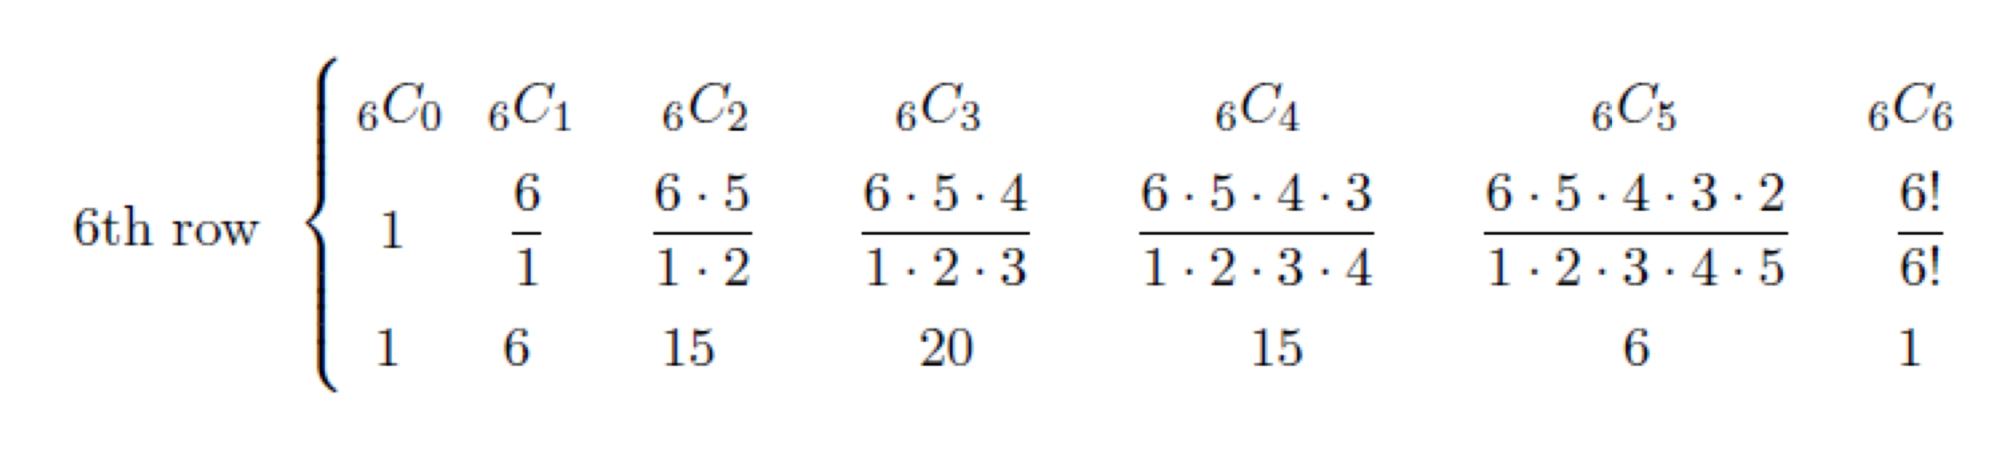
\includegraphics[width=0.6\linewidth]{./assets/binomialExpansion.png}
\end{center}

This theory is based on the Pascal's Triangle and the numbers of row $n$ correspond to the coefficients of each element of the expanded term.

We can calculate the coefficient of each part of the expanded term $k$ with combinatorics as follows: $\displaystyle {n\choose k}$

\begin{formula}[]{Binomial Expansion}
    \textbf{\textit{\underbar{In general:}}}
    \[
        (a + b)^n = 1a^nb^0 + {n\choose 1} a^{n-1}b^{1} + {n\choose 2} a^{n-2}b^{2} + \ldots + {n\choose n - 1} a^{1}b^{n - 1} + {n\choose n} a^{0}b^{n}
    \]
\end{formula}


\subsection{Overview}
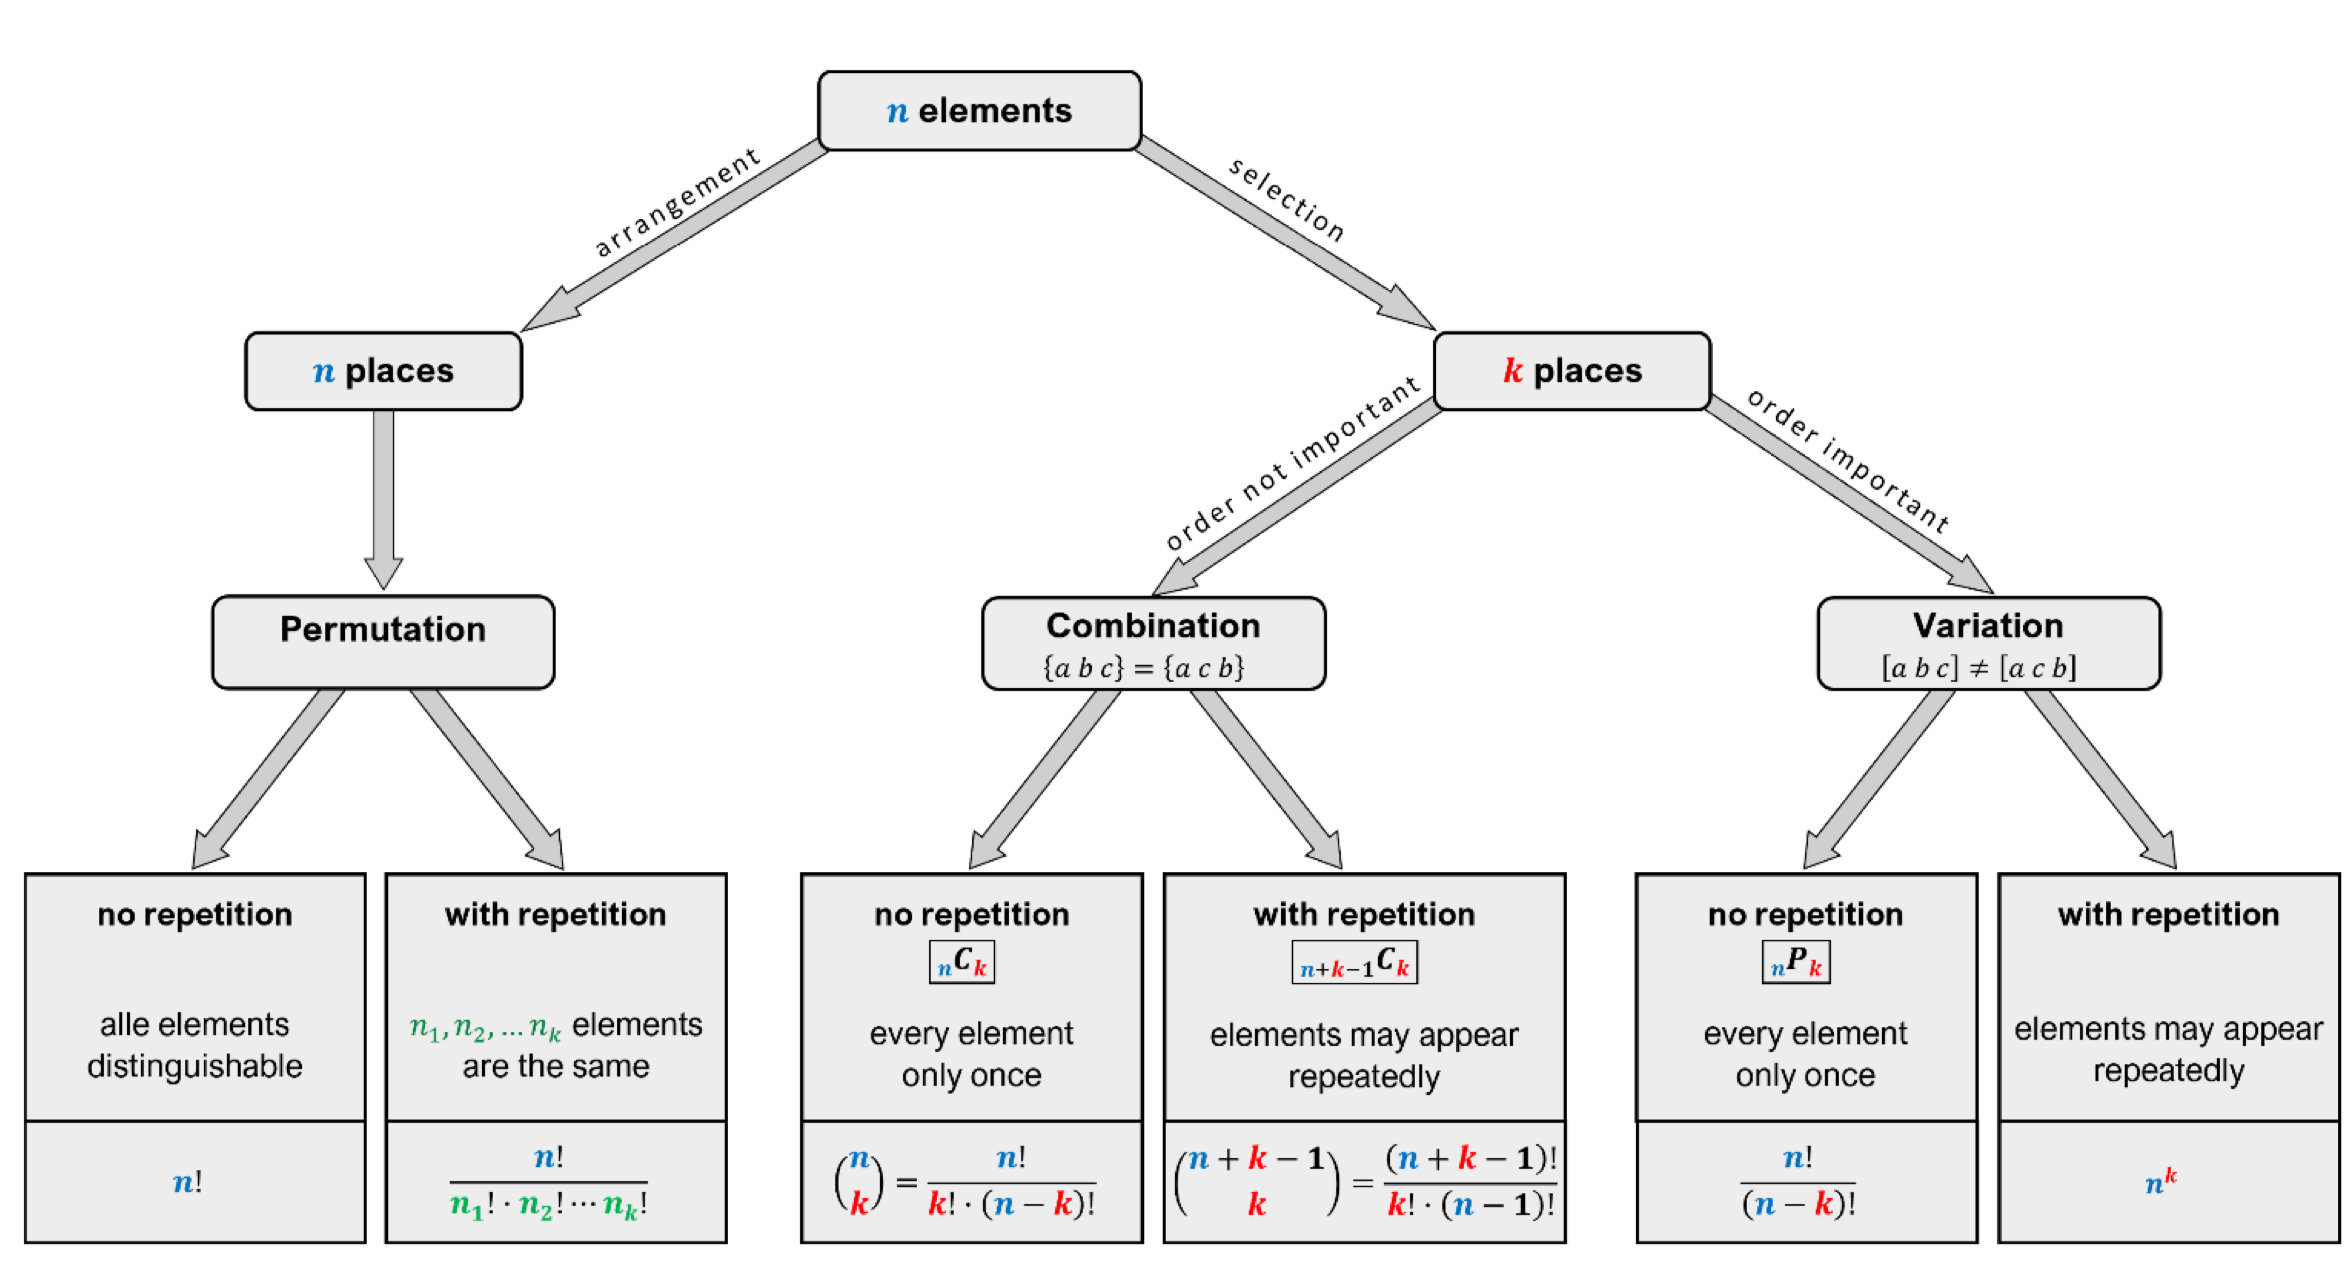
\includegraphics[width=1\linewidth]{./assets/overview.png}



\newsection
\section{Alphabete, Wörter, Sprachen und Darstellung von Problemen}
\subsection{Alphabete, Wörter, Sprachen}

\begin{definition}[]{Alphabet}
    Eine endliche, nicht leere Menge $\Sigma$. Elemente sind Buchstaben (Zeichen \& Symbole). 

    Beispiele: $\Sigma_{\text{bool}}$, $\Sigma_{\text{lat}}$ latin characters, $\Sigma_{\text{Tastatur}}$, $\Sigma_m$ $m$-adische Zahlen ($m$-ary numbers, zero index)
\end{definition}

\begin{definition}[]{Wort}
    Über $\Sigma$ eine (möglicherweise leere) Folge von Buchstaben aus $\Sigma$. Leeres Wort $\lambda$ (ab und zu $\varepsilon$) hat keine Buchstaben.

    $|w|$ ist die Länge des Wortes (Anzahl Buchstaben im Wort), während $\Sigma^*$ die Menge aller Wörter über $\Sigma$ ist und $\Sigma^+ = \Sigma^* - \{\lambda\}$

    In diesem Kurs werden Wörter ohne Komma geschrieben, also $x_1x_2\ldots x_n$ statt $x_1, x_2, \ldots, x_n$.
    Für das Leersymbol gilt $|\text{\textvisiblespace}|$, also ist es nicht dasselbe wie $\lambda$
\end{definition}

Für viele der Berechnungen in Verbindung mit der Länge der Wörter kann Kombinatorik nützlich werden. 
In Kapitel \ref{sec:combinatorics} findet sich eine Zusammenfassung über jenes Thema (in English)

Ein mögliches Alphabet beispielsweise um einen Graphen darzustellen ist folgendes: 

Angenommen, wir speichern den Graphen als Adjezenzmatrix ab, dann können wir beispielsweise mit dem Alphabet $\Sigma = \{0, 1, \#\}$ diese Matrix darstellen, in dem wir jede neue Linie mit einem $\#$ abgrenzen.
Das Problem hierbei ist jedoch, dass dies nicht so effizient ist, besonders nicht, wenn der Graph sparse ist, da wir dann viele \# im Vergleich zu nützlicher Information haben.

\begin{definition}[]{Konkatenation}
    $\Sigma^* \times \Sigma^* \rightarrow \Sigma^*$, so dass Kon$(x, y) = x \cdot y = xy \smallhspace \forall x, y \in \Sigma^*$.

    Intuitiv ist dies genau das was man denkt: Wörter zusammenhängen (wie in Programmiersprachen). 
    Die Operation ist assoziativ und hat das Neutralelement $\lambda$, was heisst, dass $(\Sigma^*, \text{Kon})$ ein Monoid ist.

    Offensichtlich ist die Konkatenation nur für ein-elementige Alphabete kommutativ.

    Die Notation $(abc)^n$ wird für die $n$-fache Konkatenation von $abc$ verwendet
\end{definition}


\begin{definition}[]{Umkehrung}
    Sei $a = a_1 a_2 \ldots a_n$, wobei $a_i \in \Sigma$ für $i \in \{1, 2, \ldots, n\}$, dann ist die Umkehrung von $a$, $a^{\text{R}} = a_n a_{n - 1} \ldots a_1$
\end{definition}


\begin{definition}[]{Iteration}
    Die $i$-te Iteration $x^i$ von $x \in \Sigma^*$ für alle $i \in \N$ ist definiert als $x^0 = \lambda$, $x^1 = x$ und $x^i = xx^{i - 1}$
\end{definition}


\begin{definition}[]{Teilwort, Präfix, Suffix}
    Seien $v, w \in \Sigma^*$
    \begin{itemize}
        \item $v$ heisst \bi{Präfix} von $w \Longleftrightarrow \exists y \in \Sigma^* : w = vy$
        \item $v$ heisst \bi{Suffix} von $w \Longleftrightarrow \exists x \in \Sigma^* : w = xv$
        \item $v$ heisst \bi{Teilwort} von $w \Longleftrightarrow \exists x, y \in \Sigma^* : w = xvy$
        \item $v \neq \lambda$ heisst \bi{echtes} Teilwort (gilt auch für Präfix, Suffix) von $w$ genau dann, wenn $v \neq w$ und $v$ ein Teilwort (oder eben Präfix oder Suffix) von $w$ ist
    \end{itemize}
\end{definition}

\begin{definition}[]{Kardinalität, Vorkommen und Potenzmenge}
    Für Wort $x \in \Sigma^*$ und Buchstabe $a \in \Sigma$ ist $|x|_a$ definiert als die Anzahl Male, die $a$ in $x$ vorkommt.

    Für jede Menge $A$ ist $|A|$ die Kardinalität und $\mathcal{P}(A) = \{S | S \subseteq A\}$ die Potenzmenge von $A$
\end{definition}


\begin{definition}[]{Kanonische Ordnung}
    Wir definieren eine Ordnung $s_1 < \ldots < s_m$ auf $\Sigma$. Die \bi{kanonische Ordnung} auf $\Sigma^*$ für $u, v \in \Sigma^*$ ist definiert als:
    \begin{align*}
        u < v \Longleftrightarrow |u| < |v| \lor (|u| = |v| \land u = x \cdot s_i \cdot u' \land v = x \cdot s_j \cdot v') \text{ für beliebige $x, u', v' \in \Sigma^*$ und $i < j$}
    \end{align*}

    Oder in Worten, geordnet nach Länge und dann danach für den ersten nicht gemeinsamen Buchstaben, nach dessen Ordnung.
\end{definition}


\begin{definition}[]{Sprache}
    $L \subseteq \Sigma^*$ ist eine Sprache, deren Komplement $L^C = \Sigma^* - L$ ist. 
    Dabei ist $L_{\emptyset}$ die \bi{leere Sprache} und $L_{\lambda}$ die einelementige Sprache die nur aus dem leeren Wort besteht.

    Die \bi{Konkatenation} von $L_1$ und $L_2$ ist $L_1 \cdot L_2 = L_1 L_2 = \{ vw \divides v \in L_1 \land w \in L_2 \}$ und $L^0 := L_{\lambda}$ und $L^{i + 1} = L^i \cdot L \smallhspace \forall i \in \N$ und $L^* = \bigcup_{i \in \N} L^{i}$ ist der \bi{Kleene'sche Stern} von $L$, wobei $L^+ = \bigcup_{i \in \N - \{0\}} L^i = L \cdot L^*$
\end{definition}

Für jede Sprache $L$ gilt $L^2 \subseteq L \Longrightarrow L = \emptyset \lor L = \{ \lambda \} \lor L$ ist undendlich. 
Diese Aussage muss jedoch an der Prüfung bewiesen werden (nicht im Buch vorhanden)

Da Sprachen Mengen sind, gelten auch die Üblichen Operationen, wie Vereinigung ($\cup$) und Schnitt ($\cap$).
Die Gleichheit von zwei Sprachen bestimmen wir weiter mit $A \subseteq B \land B \subseteq A \Rightarrow A = B$.
Um $A \subseteq B$ zu zeigen reicht es hier zu zeigen dass für jedes $x \in A$, $x \in B$ hält.
Wir betrachten nun, wie die üblichen Operationen mit der neu hinzugefügten Konkatenation interagieren.

\begin{lemma}[]{Distributivität von Kon und $\cup$}
    Für Sprachen $L_1, L_2$ und $L_3$ über $\Sigma$ gilt: $L_1 L_2 \cup L_1 L_3 = L_1 (L_2 \cup L_3)$
\end{lemma}

Der Beweis hierfür läuft über die oben erwähnte ``Regel'' zur Gleichheit. 
Um das Ganze einfacher zu machen, teilen wir auf: Wir zeigen also erst $L_1 L_2 \subseteq L_1(L_2 \cup L_3)$ und dann equivalent für $L_1 L_3$.


\begin{lemma}[]{Distributivität von Kon und $\cap$}
    Für Sprachen $L_1, L_2$ und $L_3$ über $\Sigma$ gilt: $L_1 (L_2 \cap L_3) \subseteq L_1 L_2 \cap L_1 L_3$
\end{lemma}

\shortlemma Es existieren $U_1, U_2, U_3 \in (\Sigma_{\text{bool}})^*$, so dass $U_1 (U_2 \cap U_3) \subsetneq U_1 U_2 \cap U_1 U_3$



\begin{definition}[]{Homomorphismus}
    $\Sigma_1, \Sigma_2$ beliebige Alphabete. Ein \bi{Homomorphismus} von $\Sigma^*_1$ nach $\Sigma^*_2$ ist jede Funktion $h: \Sigma_1^* \rightarrow \Sigma_2^*$ mit:
    \begin{enumerate}[label=\textit{(\roman*)}]
        \item $h(\lambda) = \lambda$
        \item $h(uv) = h(u) \cdot h(v) \smallhspace \forall u, v \in \Sigma_1^*$
    \end{enumerate}
\end{definition}

Erneut gilt hier, dass im Vergleich zu allgemeinen Homomorphismen, es zur Definition von einem Homomorphismus ausreichtt, $h(a)$ für alle Buchstaben $a \in \Sigma_1$ festzulegen.

\newpage
\subsection{Algorithmische Probleme}
Ein Algorithmus $A : \Sigma_1^* \rightarrow \Sigma_2^*$ ist eine Teilmenge aller Programme, wobei ein Program ein Algorithmus ist, sofern es für jede zulässige Eingabe eine Ausgabe liefert, es darf also nicht eine endlosschleife enthalten.

\begin{definition}[]{Entscheidungsproblem}
    Das \bi{Entscheidungsproblem} $(\Sigma, L)$ ist für jedes $x \in \Sigma^*$ zu entscheiden, ob $x \in L$ oder $x \notin L$. 
    Ein Algorithmus $A$ löst $(\Sigma, L)$ (erkennt $L$) falls für alle $x \in \Sigma^*$: $A(x) = \begin{cases}
        1, &\text{ falls } x \in L\\
        0, &\text{ falls } x \notin L
    \end{cases}$.
\end{definition}

\begin{definition}[]{Funktion}
    Algorithmus $A$ berechnet (realisiert) eine \bi{Funktion (Transformation)} $f: \Sigma^* \rightarrow \Gamma^*$ falls $A(x) = f(x) \smallhspace \forall x \in \Sigma^*$ für Alphabete $\Sigma$ und $\Gamma$
\end{definition}


\begin{definition}[]{Berechnung}
    Sei $R \subseteq \Sigma^* \times \Gamma^*$ eine Relation in den Alphabeten $\Sigma$ und $\Gamma$. 
    Ein Algorithmus $A$ \bi{berechnet} $R$ (\bi{löst das Relationsproblem} $R$) falls für jedes $x \in \Sigma^*$, für das ein $y \in \Gamma^*$ mit $(x, y) \in R$ existiert gilt:
    $(x, A(x)) \in R$
\end{definition}

\newpage
\subsection{Kolmogorov-Komplexität}
Falls ein Wort $x$ eine kürzere Darstellung hat, wird es \bi{komprimierbar genannt} und wir nennen die Erzeugung dieser Darstellung eine \bi{Komprimierung} von $x$.

Eine mögliche Idee, um den Informationsgehalt eines Wortes zu bestimmen, wäre einem komprimierbaren Wort einen kleinen Informationsgehalt zuzuordnen und einem unkomprimierbaren Wort einen grossen Informationsgehalt zuzuordnen.

Wenn wir also das Wort $011011011011011011011011$ haben, so kann man es auch als $(011)^8$ darstellen und hat so also einen kleineren Informationsgehalt als bspw. $0101101000101101001110110010$.

Die Idee mit der Komprimierung den Informationsgehalt zu bestimmen ist jedoch nicht ideal, da für jede Komprimierung bei unendlich langen Wörtern immer eine weitere Komprimierung existiert, die für unendlich viele Wörter besser geeignet ist.

Hier kommt die Kolmogorov-Komplexit zum Zuge: Sie bietet eine breit Gültige Definition des Komplexitätsmasses.


\begin{definition}[]{Kolmogorov-Komplexität}
    Für jedes Wort $x \in \wordbool$ ist die \bi{Kolmogorov-Komplexität $K(x)$ des Wortes $x$} das Minimum der binären Längen der Pascal-Programme, die $x$ generieren.
\end{definition}

Hierbei ist mit der binären Länge die Anzahl Bits gemeint, die beim Übersetzen des Programms in einen vordefinierten Maschinencode entsteht.

Ein Pascal-Programm in diesem Kurs ist zudem nicht zwingend ein Programm in der effektiven Programmiersprache Pascal, sondern eine Abwandlung davon, worin es auch erlaubt ist, gewisse Prozesse zu beschreiben und nicht als Code auszuformulieren, da das nicht das Ziel dieses Kurses ist.


\begin{lemma}[]{Kolmogorov-Komplexität}
    Für jedes Wort $x \in \wordbool$ existiert eine Konstante $d$ so dass $K(x) \leq |x| + d$
\end{lemma}
\inlineproof Für jedes $x \in \wordbool$ kann folgendes Programm $A_x$ verwendet werden:

\begin{minted}{pascal}
A_x: begin
        write(x);
     end
\end{minted}
Alle Teile, ausser $x$ sind dabei von konstanter Länge, also ist die Länge der Bit-repräsentation des Programms ausschliesslich von der binären Länge des Wortes $x$ abhängig.

\proven


Für regelmässige Wörter gibt es natürlich Programme, bei denen das Wort nicht als komplette Variable vorkommt. 
Deshalb haben diese Wörter auch (meist) eine kleinere Kolmogorov-Komplexität.


\fancydef{$K(n)$ für $n \in \N$} Die \bi{Kolmogorov-Komplexität einer natürlichen Zahl $n$} ist $K(n) = K(\text{Bin}(n))$,
wobei $\text{Bin}(x) = \ceil{\log_2(x + 1)}$ % TODO: Verify correctness here





\end{document}
